%\usetikzlibrary{matrix}
\begin{tikzpicture}[x=0.5cm, y=0.4cm] [
	cnn/.pic={
		\draw (0,0) rectangle (0.5,0.55);
	}
]

	  \matrix (m) [matrix of nodes, 
    column sep=5mm,
    row sep=1cm,
    nodes={draw, % General options for all nodes
      line width=1pt,
      anchor=center, 
      text centered,
      %rounded corners,
      minimum width=1.5cm, minimum height=8mm
    }, 
    % Define styles for some special nodes
    right iso/.style={isosceles triangle,scale=0.5,sharp corners, anchor=center, xshift=-4mm},
    left iso/.style={right iso, rotate=180, xshift=-8mm},
    txt/.style={text width=1.5cm,anchor=center},
    ellip/.style={ellipse,scale=0.5},
    empty/.style={draw=none}
    ]
  {
  %Row 1
   &   \begin{tikzpicture} \draw (-0.1,-0.3) rectangle ++(0.5,0.5); \draw (0.6,0.6) rectangle ++(0.4, -0.4);
  \draw (0.8,0.3) rectangle ++(0.4, -0.4);
  \draw (1.2,-0.3) rectangle ++(0.4, -0.4);  
  \draw (2, 0.3) rectangle ++(0.3, -0.8);
  \draw[-latex] (0.4, -0.05) -- ++(0.3, 0);
  \end{tikzpicture} & Addition &  & 
  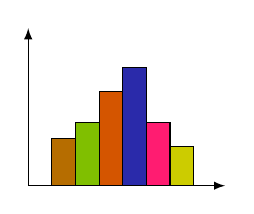
\begin{tikzpicture}
  	\draw[-latex] (0,0) -- (2.5,0);
  	\draw[-latex] (0,0) -- (0,2);  	
  	\foreach \i/\h/\c in {1/0.6/{rgb:red,4;green,2;yellow,1},2/0.8/{rgb:red,1;green,2;yellow,1},3/1.2/{rgb:red,4;green,1;yellow,1},4/1.5/{rgb:red,1;green,1;blue,4},5/0.8/{rgb:red,4;magenta,4;yellow,1},6/0.5/{rgb:red,1;green,1;yellow,3}}
  	{
  		\draw[fill={\c}] (0.3*\i, 0) rectangle ++(0.3, \h);
  	}
  \end{tikzpicture}  
  &  &  & \\
$v_{i,1}$ & & & & & Fusion layer&

  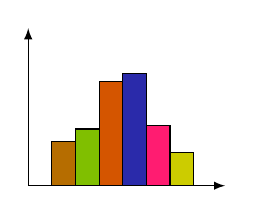
\begin{tikzpicture}
  	\draw[-latex] (0,0) -- (2.5,0);
  	\draw[-latex] (0,0) -- (0,2);  	
  	\foreach \i/\h/\c in {1/0.56/{rgb:red,4;green,2;yellow,1},2/0.72/{rgb:red,1;green,2;yellow,1},3/1.32/{rgb:red,4;green,1;yellow,1},4/1.42/{rgb:red,1;green,1;blue,4},5/0.76/{rgb:red,4;magenta,4;yellow,1},6/0.42/{rgb:red,1;green,1;yellow,3}}
  	{
  		\draw[fill={\c}] (0.3*\i, 0) rectangle ++(0.3, \h);
  	}
  \end{tikzpicture}  

 \\
%Row 3
&
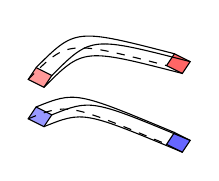
\begin{tikzpicture}
	\draw[fill=red!40] (0,0) coordinate (a) -- ++(0.2, -0.1) coordinate (b) -- ++(0.1, 0.15) coordinate (c) -- ++(-0.2, 0.1) coordinate (d) -- cycle;
	\draw[fill=blue!40]  (0,-0.5) coordinate (i) -- ++(0.2, -0.1) coordinate (j) -- ++(0.1, 0.15) coordinate (k) -- ++(-0.2, 0.1) coordinate (l) -- cycle;
	\begin{scope}[xshift=50, yshift=5]
		\draw[fill=red!60]  (0,0) coordinate (e) -- ++(0.2, -0.1) coordinate (f) -- ++(0.1, 0.15) coordinate (g) -- ++(-0.2, 0.1) coordinate (h) -- cycle;
		\draw[fill=blue!60]  (0,-1) coordinate (m) -- ++(0.2, -0.1) coordinate (n) -- ++(0.1, 0.15) coordinate (o) -- ++(-0.2, 0.1) coordinate (p) -- cycle;		
	\end{scope}
	\draw[dashed] (a) .. controls (0.5,0.5) ..  (e);
	\draw (b) .. controls (0.7,0.4) ..  (f);
	\draw (c) .. controls (0.8,0.55) ..  (g);
	\draw (d) .. controls (0.6,0.65) ..  (h);
	
	\draw[dashed] (i) .. controls (0.5,-0.3) ..  (m);
	\draw (j) .. controls (0.7,-0.4) ..  (n);
	\draw (k) .. controls (0.8, -0.25) ..  (o);
	\draw (l) .. controls (0.6, -0.15) ..  (p);	
\end{tikzpicture}
& 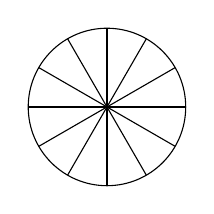
\begin{tikzpicture}
	\draw (0,0) circle (1);
	\foreach \a in {0, 1, 2, 3, 4, 5}
	{
		\draw (\a*30:1) -- ++(\a*30:-2);
	}
\end{tikzpicture} &
BoW &
  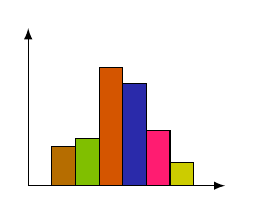
\begin{tikzpicture}
  	\draw[-latex] (0,0) -- (2.5,0);
  	\draw[-latex] (0,0) -- (0,2);  	
  	\foreach \i/\h/\c in {1/0.5/{rgb:red,4;green,2;yellow,1},2/0.6/{rgb:red,1;green,2;yellow,1},3/1.5/{rgb:red,4;green,1;yellow,1},4/1.3/{rgb:red,1;green,1;blue,4},5/0.7/{rgb:red,4;magenta,4;yellow,1},6/0.3/{rgb:red,1;green,1;yellow,3}}
  	{
  		\draw[fill={\c}] (0.3*\i, 0) rectangle ++(0.3, \h);
  	}
  \end{tikzpicture}  
\\

$v_{i,n}$ & & & & & & & &

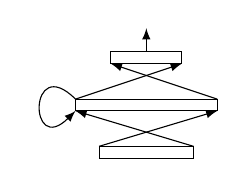
\begin{tikzpicture}[scale=0.3]
	\draw  (0,0) -- ++(2, 0) -- ++(0, 0.5) coordinate  (a)  -- ++(-4, 0) coordinate  (b) -- ++(0, -0.5) -- cycle;
	
	
	\draw  (0,2) -- ++(3, 0) coordinate  (c) -- ++(0, 0.5) coordinate (d)  -- ++(-6, 0) coordinate  (e) -- ++(0, -0.5)  coordinate  (f)  -- cycle;
	
	\draw  (0,4) -- ++(1.5, 0)  coordinate  (g) -- ++(0, 0.5)  -- ++(-3, 0) coordinate[midway] (t) -- ++(0, -0.5) coordinate  (h) -- cycle;	
	
	\draw[-latex] (a) -- (f);
	\draw[-latex] (b) -- (c);
	
	\draw[-latex] (e) -- (g);
	\draw[-latex] (d) -- (h);	
	
	\draw[-latex] (t) -- ++(0, 1);		
	\draw[-latex] (e)  .. controls ++(-2,2) and ++(-2, -2) ..  (f);
\end{tikzpicture} 
\\
  };
  
  \node at (m-1-2) [anchor=south, yshift=25] {CNN};
  \node at (m-3-3) [anchor=south, yshift=35] {HOOF};
    \node at (m-4-9) [anchor=south, yshift=30] {LSTM network};
        \node at (m-1-5) [anchor=south, yshift=35] {Static vector};
        \node at (m-3-5) [anchor=south, yshift=35] {Motion vector};        
        \node at (m-3-2) [anchor=south, yshift=30] {Motion tubes};               
  
  \draw[-latex] (m-2-1) |- (m-1-2);
  \draw[-latex] (m-2-1) |- (m-3-2);
  
    \draw[-latex] (m-1-2) -- (m-1-3);
  \draw[-latex] (m-3-2) -- (m-3-3);
  
   \draw[-latex] (m-1-3) --(m-1-5);
  \draw[-latex] (m-3-3) -- (m-3-4);
    \draw[-latex] (m-3-4) --  (m-3-5);
    
     \draw[-latex] (m-1-5) -| (m-2-6);
    \draw[-latex] (m-3-5) -|  (m-2-6);
    
\draw[-latex] (m-2-6) -- (m-2-7);

\draw[-latex] (m-2-7) |- ($(m-4-9.west)+(0, 0.8)$);
\draw[-latex] ($(m-4-9.west)+(-2.4, 0.4)$) -- ++(2.4, 0);
\draw[-latex] ($(m-4-9.west)+(-2.4, 0)$) -- ++(2.4, 0);
\node at ($(m-4-9.west)+(-2.4, -0.25)$) {$\vdots$}; 
\draw[-latex] ($(m-4-9.west)+(-2.4, -0.8)$) -- ++(2.4, 0);

\node at ($(m-4-1)+(0, 1)$) {$\vdots$}; 
\node at ($(m-4-1)+(5, 0)$) {$\cdots$}; 

\draw[-latex] (m-4-9) -- ++(2,0) node [anchor=west] {Classification};
  
\end{tikzpicture}